\subsection{Basic Block Vectors}

Basic block vectors (BBV)~\cite{Sherwood:2003:DEP} encodes the execution frequency of basic blocks over an interval. BBVs can be approximated using an array of accumulators (counters) that tracks the number of instructions executed by a basic block in a given execution interval (see Figure~\ref{fig:bbv}). When a branch PC is encountered, a hash function is applied to the PC to determine an index into the accumulator table in order to increment the appropriate counter by the number of committed instructions since the last branch instruction. The BBV difference between intervals is computed using the manhattan distance. A phase change is determined by comparing the BBV difference to a difference threshold. The hardware required to implement BBVs includes an N-bit wide RAM array for the accumulator table, sampling hardware to detect branch instructions and analyze the retire stream, and an N-bit adder to update the accumulator table. The hardware complexity of BBV is much higher compared to working set signatures. 

\begin{figure}[htbp]
  \begin{center}
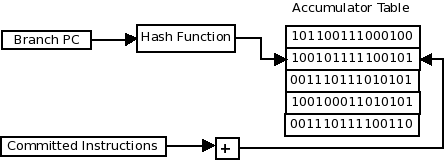
\includegraphics[width=0.80\columnwidth]{figs/bbv}
  \end{center}
  \caption{BBV accumulator table update technique.}
  \label{fig:bbv}
\end{figure}
